\chapter{分离与可数}

\section{正则空间和正规空间}
\begin{definition}[正则空间]
    一个拓扑空间 $X$ 称为\textbf{正则的}, 如果
    \begin{enumerate}
        \item[(i)] $X$ 中的单点集是闭集;
        \item[(ii)] 对任意 $a \in X$ 和 $X$ 中的任意闭集 $B$ 且 $a \notin B$, 存在不相交的开集 $U$ 和 $V$ 使得 $a \in U$ 且 $B \subset V$.
    \end{enumerate}
\end{definition}
\begin{figure}[h]
    \centering
    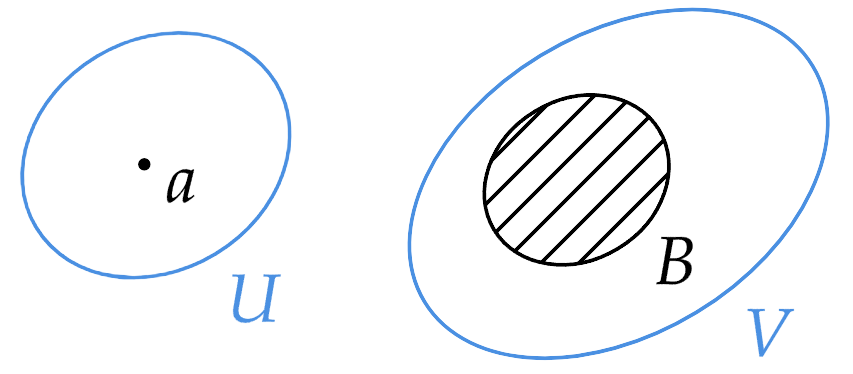
\includegraphics[width=0.35\textwidth]{fig/5.1.png}
    \caption{正则空间}
\end{figure}

\begin{remark}
    正则 $\implies$ Hausdorff.
\end{remark}

\begin{definition}[正规空间]
    一个拓扑空间 $X$ 称为\textbf{正规的}, 如果
    \begin{enumerate}
        \item[(i)] $X$ 中的单点集是闭集;
        \item[(ii)] 对任意两个不相交的闭集 $A, B \subset X$, 存在不相交的开集 $U$ 和 $V$ 使得 $A \subset U$ 且 $B \subset V$.
    \end{enumerate}
\end{definition}
\begin{figure}[h]
    \centering
    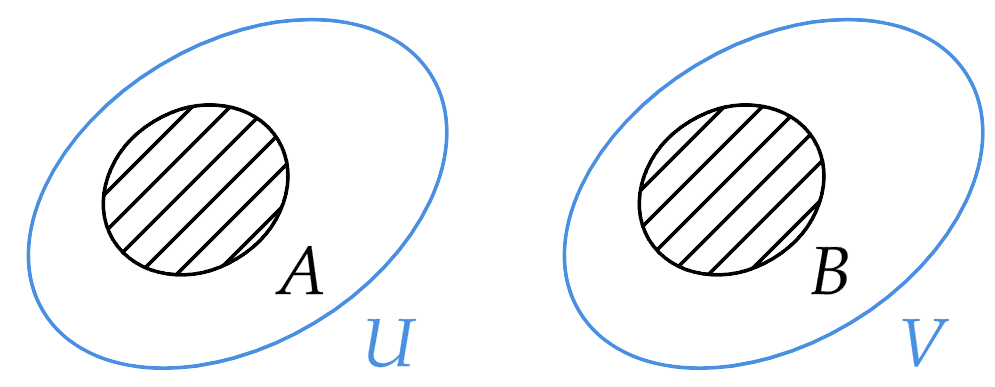
\includegraphics[width=0.35\textwidth]{fig/5.2.png}
    \caption{正规空间}
\end{figure}

\begin{remark}
    正规 $\implies$ 正则.
\end{remark}

\section{分离公理}

我们也称 Hausdorff 空间为 $T_2$ 空间, 正则空间为 $T_3$ 空间, 正规空间为 $T_4$ 空间，它们都反应了拓扑空间的分离性质，并且有以下包含关系:
\begin{axiom}{分离公理}
    正规 ($T_4$) $\subset$ 正则 ($T_3$) $\subset$ Hausdorff ($T_2$)
\end{axiom}

上一节章中证明了每个度量空间都是 Hausdorff 的，现在可以进一步证明每个度量空间都是正规的，也就是度量空间有最强的分离性质.\par
\begin{proposition}
    任意一个度量空间都是正规的.
\end{proposition}
\begin{proof}
    首先，对$\forall\, x\in X,y\in X-\{x\}$，$d(x,y)>0$，则$y\in B\left(y,d(x,y)\right)\subset X-\{x\}$，因此$X-\{x\}$是一个开集，从而单点集$\{x\}$是闭集.\par
    假设 $X$ 是一个度量空间, $A$ 和 $B$ 是 $X$ 中两个不相交的闭集.定义如下函数：
    {\setjot[-7]\begin{align*}
        g: X &\to \mathbb{E}^1 \\ 
        x &\mapsto d(x, A) := \inf\{d(x, a) \mid a \in A\} \\
        h: X &\to \mathbb{E}^1 \\ 
        x &\mapsto d(x, B) := \inf\{d(x, b) \mid b \in B\} \\
        f: X &\to \mathbb{E}^1 \\
        x &\mapsto \frac{d(x, A)}{d(x, A) + d(x, B)}
    \end{align*}}\par
    \hspace{-1.5em}(i)\; 证明 $g$ 和 $h$ 是连续的.即对$\forall\,(r, s) \subset \mathbb{E}^1$, $g^{-1}((r, s))$ 在 $X$ 中是开集.\par
    也就是$\forall\,x \in g^{-1}((r, s))$，我们需要证明$\exists\,\varepsilon > 0$ 使得 $x \in B(x, \varepsilon) \subset g^{-1}((r, s))$.
    \begin{center}
        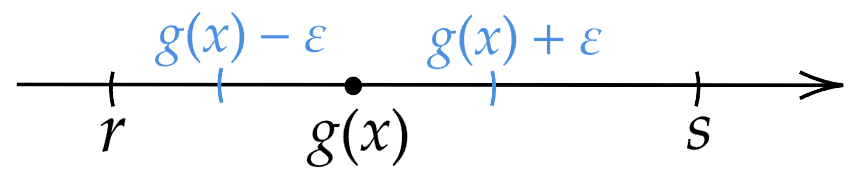
\includegraphics[width=0.35\textwidth]{fig/5.3.png}
        \captionof{figure}{}
    \end{center}\par
    由$g(x) \in (r, s)$，可取$\varepsilon > 0$ 使得$(g(x)-\varepsilon, g(x)+\varepsilon) \subset (r, s)$，即 $g(x)-\varepsilon > r$ 且 $g(x)+\varepsilon < s$.\par        
    那么$\forall\,y \in B(x, \varepsilon)$，有$d(x, y) < \varepsilon$，则$\setjot[-4]\begin{aligned}[t]
        g(y) &= d(y, A) = \inf\{d(y, a) \mid a \in A\}  \\
        &\leq \inf\{d(y, x) + d(x, a) \mid a \in A\} \\
        &= d(y, x) + d(x, A) < \varepsilon + g(x) < s
        \end{aligned}$.\par
    另一方面，$g(x) = d(x, A) \leq d(x, y) + d(y, A) < \varepsilon + g(y) \implies g(y) > g(x) - \varepsilon > r$.\par
    因此 $g(y) \in (r, s)$, 所以 $B(x, \varepsilon) \subset g^{-1}((r, s))$.
    这证明了 $g^{-1}((r, s))$ 是开集, 所以 $g$ 是连续的.\par
    同理, $h$ 也是连续的.\par
    \hspace{-1.8em}(ii)\; 证明$\forall\,x \in X$, $d(x, A) + d(x, B) > 0$.
    等价于证明 $d(x, A) + d(x, B) \neq 0$.\par
    \begin{minipage}[t]{0.765\textwidth}
         先证$d(x, A) = 0 \iff x \in A$.\par
    “$\Leftarrow$”显然.\par
    “$\Rightarrow$”设$x\notin A$.由于$A$是闭集，$X-A$是开集，故$\exists\, \delta>0,\st B(x,\delta)\subset X-A$.\par
    则$d(x,A)\geq \delta>0$，矛盾!\par
    \end{minipage}
    \begin{minipage}[t]{0.18\textwidth}
        \vspace{-3em}
        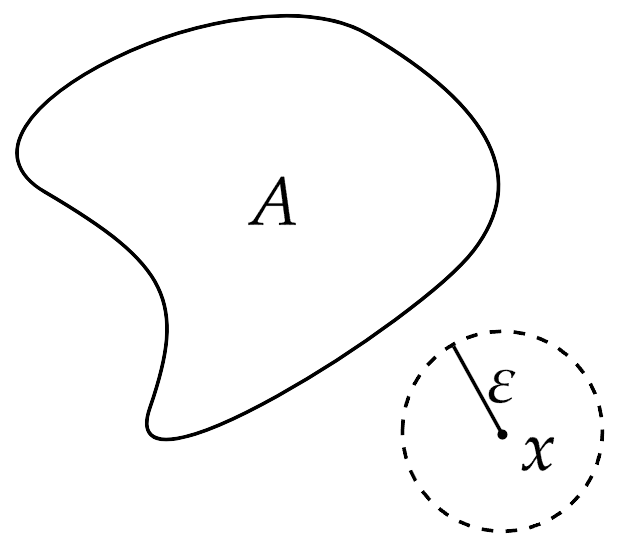
\includegraphics[width=1\textwidth]{fig/5.4.png}
        \captionof{figure}{}
    \end{minipage}\par
    如果 $d(x, A) + d(x, B) = 0$, 那么必有 $d(x, A) = 0$ 和 $d(x, B) = 0$. \par
    这意味着 $x \in A$ 且 $x \in B$, 即 $x \in A \cap B$.但这与 $A \cap B = \varnothing$ 矛盾.\par
    (ii)证明了$f$的分母恒不为零.\par    
    由 (i) 和 (ii), 函数 $f$ 是连续的 (因为它是连续函数的和、商, 且分母不为零).\par
    对$\forall\,a \in A$，$d(a,A)=0$，故$f(a) = \frac{d(a, A)}{d(a, A) + d(a, B)} = \frac{0}{0 + d(a, B)} = 0$.\par
    对任意 $b \in B$，$d(b,B)=0$，故$f(b) = \frac{d(b, A)}{d(b, A) + d(b, B)} = \frac{d(b, A)}{d(b, A) + 0} = 1$.\par
    令 $U = f^{-1}\left(\left(-\infty, \frac{1}{2}\right)\right)$ 和 $V = f^{-1}\left(\left(\frac{1}{2},+\infty\right)\right)$.
    因为 $f$ 是连续的, $U$ 和 $V$ 都是开集.
    并且 $A \subset U$, $B \subset V$, 且 $U \cap V = \varnothing$.
    这就证明了 $X$ 是正规空间.
\end{proof}

\section{可数性}
\begin{definition}[可数邻域基]
    设$X$是一个拓扑空间，$x\in X$，如果存在$x$的一个可数邻域族$\{U_n\}_{n \in \mathbb{Z}^+}$，使得$x$的任何邻域 $W$都包含其中一个 $U_n$, 即 $x \in U_n \subset W$，则称在点$x$处一个\textbf{可数邻域基}.
\end{definition}
\vspace{-1.5 em}
\begin{figure}[h]
    \centering
    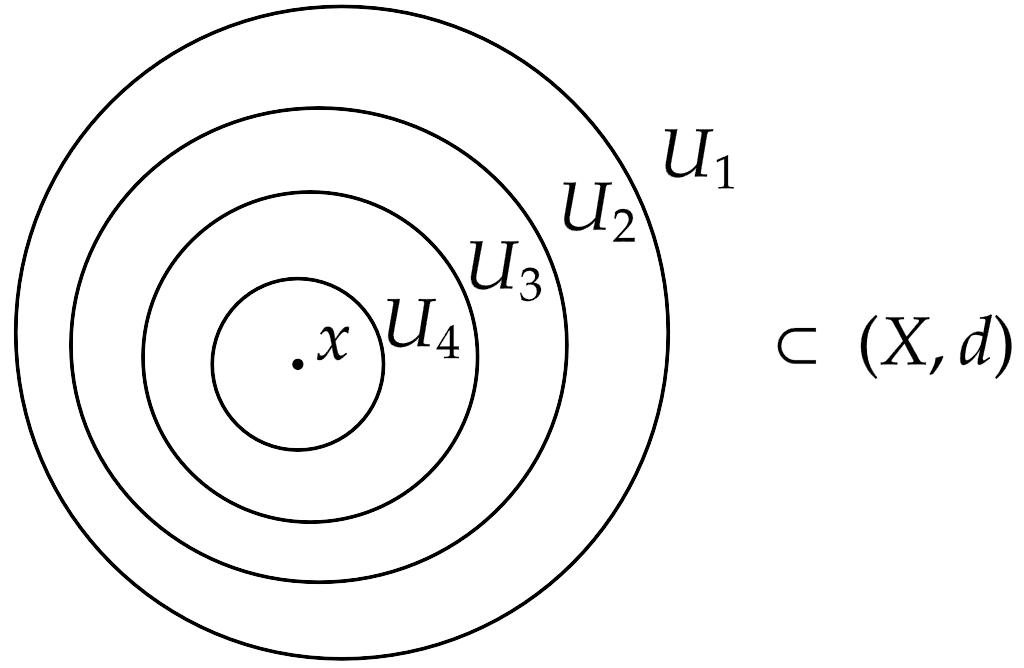
\includegraphics[width=0.3\textwidth]{fig/5.5.png}
    \caption{可数邻域基}
\end{figure}

\begin{definition}[第一可数]
    如果 $X$ 在其每一点都有可数邻域基, 则称 $X$ 是\textbf{第一可数的}，记为$C_1$空间.
\end{definition}

\begin{instance}
    每个度量空间都是第一可数的.\par
    对$\forall\,x \in (X, d)$, $\left\{U_n = B\left(x, \frac{1}{n}\right)\right\}_{n \in \mathbb{Z}^+}$ 是一个可数邻域基.
\end{instance}

\begin{definition}[第二可数]
    设$X$是一个拓扑空间，若$X$有一个可数基, 则称$X$是\textbf{第二可数的}, 记为$C_2$空间.
\end{definition}

\begin{instance}
    $\mathbb{E}^n$ 是第二可数的.一个可数基是 $\mathcal{B} = \left\{B\left(x, \frac{1}{k}\right) \Big| x \in \mathbb{Q}^n, k \in \mathbb{Z}^+\right\}$.\par
    \begin{enumerate}
        \item $B \left(x,\frac{1}{k}\right)$是$\mb{E}^n$中的开集.
        \item 对任意开集$U\subset \mb{E}^n$，$\forall\,x\in U$，$\exists\, \delta>0,\st x\in B(x,\delta)\subset U$，可以在$U$中找到一个距离$x$很近的$\tilde{x}$，且$d(x,\tilde{x})=\frac{1}{k_1},k_1\in\mb{Z}$，则$x\in B\left(x,\frac{1}{k_1}\right)\subset B(x,\delta)\subset U$.\par
    \end{enumerate}
\end{instance}

\begin{proposition}
    每个第二可数空间都是第一可数的.
\end{proposition}
\begin{proof}
    假设$X$是第二可数的，$\mathcal{B}$是$X$的一个可数基.\par
    $\forall\, x\in X$，$\{B\in\mcal{B}|x\in B\}$是$x$的一个可数邻域基.可数性自然可得，下证其确实为邻域基.\par
    对任意$x$的邻域$W$，$\exists\, B_1\in\mcal{B},\st x\in B_1\subset W$.
\end{proof}

\begin{instance}
    考虑$\mb{R}$上的离散拓扑，则它不是第二可数的.这是因为其中的单点集都是开集，因此必须是基元素，故而基必然不可数.\par
    但这个拓扑空间是可度量化的，其度量为离散度量.\par
\end{instance}
从上述例子中可以看出，度量空间虽然是正规的、第一可数的，但它不一定是第二可数的，因此第二可数空间是极强的条件.\par

\begin{proposition}
    \begin{enumerate}[(i)]
        \item 第一（第二）可数空间的子空间是第一（第二）可数的.
        \item 两个第一（第二）可数空间的乘积是第一（第二）可数的.
    \end{enumerate}
\end{proposition}
\begin{proof}
    对于第二可数的情况：
    \begin{enumerate}
        \item[(i)] 设 $X$ 是第二可数的，$\mathcal{B}$ 是 $X$ 的一个可数基.设 $A \subset X$ 是一个子空间，则 $\mathcal{B}_A = \{B \cap A \mid B \in \mathcal{B}\}$ 是 $A$ 的一个可数基.
        \item[(ii)] 设 $X_1, X_2$ 是第二可数空间，$\mathcal{B}_i$ 是 $X_i$ 的可数基，$i=1,2$.则 $\mathcal{B} = \{B_1 \times B_2 \mid B_1 \in \mathcal{B}_1, B_2 \in \mathcal{B}_2\}$ 是 $X_1 \times X_2$ 的一个可数基.
    \end{enumerate}
\end{proof}

\section{两个定理}
\begin{theorem}[Urysohn 度量化定理]
    如果一个拓扑空间 $X$ 是正则的且是第二可数的，那么 $X$ 是可度量化的.
    \[
        \left.
        \begin{array}{r}
            \text{正则} \\
            \text{第二可数}
        \end{array}
        \right\} \implies \text{可度量化}
    \]
\end{theorem}
反过来，对于度量空间，我们只能得到正规和第一可数的条件.

\begin{theorem}[Tietze 扩张定理]
    如果 $X$ 是一个正规空间，$A \subset X$ 是闭集，$f: A \to \mathbb{E}^1$ 是一个连续函数.那么存在一个连续函数 $F: X \to \mathbb{E}^1$ 使得对所有 $a \in A$ 都有 $F(a) = f(a)$.
\end{theorem}

\begin{instance}
    在 $\mathbb{Z}$ 上，令 $\mathcal{B} := \{B_{a,b} = \{a+nb : n \in \mathbb{Z}\} \mid a,b \in \mathbb{Z}, b>0\}$ 作为基.这个基生成一个度量拓扑.
    \begin{enumerate}
        \item[(i)] $B_{0,b}, B_{1,b}, \dots, B_{b-1,b}$ 覆盖 $\mathbb{Z}$.
        \item[(ii)] $x \in B_{a_1, b_1} \cap B_{a_2, b_2}$.
    \end{enumerate}
    它是第二可数的，因为基 $\mathcal{B}$ 是可数的.
    \paragraph{它是正则的}
    \begin{enumerate}
        \item[(a)] 对任意 $z \in \mathbb{Z}$，$\{z\}$ 是闭集.
        对任意 $a \in \mathbb{Z} - \{z\}$，选择整数 $b > |a-z|$.那么 $a \in B_{a,b} \subset \mathbb{Z} - \{z\}$.\par
        \begin{center}
            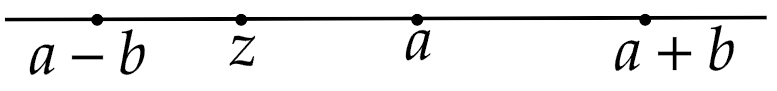
\includegraphics[width=0.35\textwidth]{fig/5.6.png}
            \captionof{figure}{}
        \end{center}
        \item[(b)] 对任意 $z \in \mathbb{Z}$，任意闭集 $C \subset \mathbb{Z}$ 且 $z \notin C$.存在 $B_{a,b}$ 使得 $z \in B_{a,b} \subset \mathbb{Z} - C$.
        事实上，$B_{a,b}$ 既是开集也是闭集.
        $\mathbb{Z} - B_{a,b} = \bigcup_{a' \not\equiv a \pmod b} B_{a',b}$ 是开集. \par
        $\mb{Z}-B_{1,3}=B_{0,3}\cup B_{2,3}$.\par
        令$U=B_{a,b},V=\mb{Z}-B_{a,b}$，则$U\cap V=\varnothing$，$U,V$都是开集，且$z\in U,C\subset V$.
    \end{enumerate}
\end{instance}




